% Created 2019-12-16 Mon 23:42
% Intended LaTeX compiler: pdflatex
\documentclass[12pt]{article}
\usepackage[utf8]{inputenc}
\usepackage[T1]{fontenc}
\usepackage{graphicx}
\usepackage{longtable}
\usepackage{wrapfig}
\usepackage{rotating}
\usepackage[normalem]{ulem}
\usepackage{amsmath}
\usepackage{textcomp}
\usepackage{amssymb}
\usepackage{capt-of}
\usepackage{hyperref}
\usepackage{minted}
\ifdefined\orglatexfragmentpreview
\else
\usepackage{iclr2020_conference,times}
%%%%% NEW MATH DEFINITIONS %%%%%

\usepackage{amsmath,amsfonts,bm}

% Mark sections of captions for referring to divisions of figures
\newcommand{\figleft}{{\em (Left)}}
\newcommand{\figcenter}{{\em (Center)}}
\newcommand{\figright}{{\em (Right)}}
\newcommand{\figtop}{{\em (Top)}}
\newcommand{\figbottom}{{\em (Bottom)}}
\newcommand{\captiona}{{\em (a)}}
\newcommand{\captionb}{{\em (b)}}
\newcommand{\captionc}{{\em (c)}}
\newcommand{\captiond}{{\em (d)}}

% Highlight a newly defined term
\newcommand{\newterm}[1]{{\bf #1}}


% Figure reference, lower-case.
\def\figref#1{figure~\ref{#1}}
% Figure reference, capital. For start of sentence
\def\Figref#1{Figure~\ref{#1}}
\def\twofigref#1#2{figures \ref{#1} and \ref{#2}}
\def\quadfigref#1#2#3#4{figures \ref{#1}, \ref{#2}, \ref{#3} and \ref{#4}}
% Section reference, lower-case.
\def\secref#1{section~\ref{#1}}
% Section reference, capital.
\def\Secref#1{Section~\ref{#1}}
% Reference to two sections.
\def\twosecrefs#1#2{sections \ref{#1} and \ref{#2}}
% Reference to three sections.
\def\secrefs#1#2#3{sections \ref{#1}, \ref{#2} and \ref{#3}}
% Reference to an equation, lower-case.
\def\eqref#1{equation~\ref{#1}}
% Reference to an equation, upper case
\def\Eqref#1{Equation~\ref{#1}}
% A raw reference to an equation---avoid using if possible
\def\plaineqref#1{\ref{#1}}
% Reference to a chapter, lower-case.
\def\chapref#1{chapter~\ref{#1}}
% Reference to an equation, upper case.
\def\Chapref#1{Chapter~\ref{#1}}
% Reference to a range of chapters
\def\rangechapref#1#2{chapters\ref{#1}--\ref{#2}}
% Reference to an algorithm, lower-case.
\def\algref#1{algorithm~\ref{#1}}
% Reference to an algorithm, upper case.
\def\Algref#1{Algorithm~\ref{#1}}
\def\twoalgref#1#2{algorithms \ref{#1} and \ref{#2}}
\def\Twoalgref#1#2{Algorithms \ref{#1} and \ref{#2}}
% Reference to a part, lower case
\def\partref#1{part~\ref{#1}}
% Reference to a part, upper case
\def\Partref#1{Part~\ref{#1}}
\def\twopartref#1#2{parts \ref{#1} and \ref{#2}}

\def\ceil#1{\lceil #1 \rceil}
\def\floor#1{\lfloor #1 \rfloor}
\def\1{\bm{1}}
\newcommand{\train}{\mathcal{D}}
\newcommand{\valid}{\mathcal{D_{\mathrm{valid}}}}
\newcommand{\test}{\mathcal{D_{\mathrm{test}}}}

\def\eps{{\epsilon}}


% Random variables
\def\reta{{\textnormal{$\eta$}}}
\def\ra{{\textnormal{a}}}
\def\rb{{\textnormal{b}}}
\def\rc{{\textnormal{c}}}
\def\rd{{\textnormal{d}}}
\def\re{{\textnormal{e}}}
\def\rf{{\textnormal{f}}}
\def\rg{{\textnormal{g}}}
\def\rh{{\textnormal{h}}}
\def\ri{{\textnormal{i}}}
\def\rj{{\textnormal{j}}}
\def\rk{{\textnormal{k}}}
\def\rl{{\textnormal{l}}}
% rm is already a command, just don't name any random variables m
\def\rn{{\textnormal{n}}}
\def\ro{{\textnormal{o}}}
\def\rp{{\textnormal{p}}}
\def\rq{{\textnormal{q}}}
\def\rr{{\textnormal{r}}}
\def\rs{{\textnormal{s}}}
\def\rt{{\textnormal{t}}}
\def\ru{{\textnormal{u}}}
\def\rv{{\textnormal{v}}}
\def\rw{{\textnormal{w}}}
\def\rx{{\textnormal{x}}}
\def\ry{{\textnormal{y}}}
\def\rz{{\textnormal{z}}}

% Random vectors
\def\rvepsilon{{\mathbf{\epsilon}}}
\def\rvtheta{{\mathbf{\theta}}}
\def\rva{{\mathbf{a}}}
\def\rvb{{\mathbf{b}}}
\def\rvc{{\mathbf{c}}}
\def\rvd{{\mathbf{d}}}
\def\rve{{\mathbf{e}}}
\def\rvf{{\mathbf{f}}}
\def\rvg{{\mathbf{g}}}
\def\rvh{{\mathbf{h}}}
\def\rvu{{\mathbf{i}}}
\def\rvj{{\mathbf{j}}}
\def\rvk{{\mathbf{k}}}
\def\rvl{{\mathbf{l}}}
\def\rvm{{\mathbf{m}}}
\def\rvn{{\mathbf{n}}}
\def\rvo{{\mathbf{o}}}
\def\rvp{{\mathbf{p}}}
\def\rvq{{\mathbf{q}}}
\def\rvr{{\mathbf{r}}}
\def\rvs{{\mathbf{s}}}
\def\rvt{{\mathbf{t}}}
\def\rvu{{\mathbf{u}}}
\def\rvv{{\mathbf{v}}}
\def\rvw{{\mathbf{w}}}
\def\rvx{{\mathbf{x}}}
\def\rvy{{\mathbf{y}}}
\def\rvz{{\mathbf{z}}}

% Elements of random vectors
\def\erva{{\textnormal{a}}}
\def\ervb{{\textnormal{b}}}
\def\ervc{{\textnormal{c}}}
\def\ervd{{\textnormal{d}}}
\def\erve{{\textnormal{e}}}
\def\ervf{{\textnormal{f}}}
\def\ervg{{\textnormal{g}}}
\def\ervh{{\textnormal{h}}}
\def\ervi{{\textnormal{i}}}
\def\ervj{{\textnormal{j}}}
\def\ervk{{\textnormal{k}}}
\def\ervl{{\textnormal{l}}}
\def\ervm{{\textnormal{m}}}
\def\ervn{{\textnormal{n}}}
\def\ervo{{\textnormal{o}}}
\def\ervp{{\textnormal{p}}}
\def\ervq{{\textnormal{q}}}
\def\ervr{{\textnormal{r}}}
\def\ervs{{\textnormal{s}}}
\def\ervt{{\textnormal{t}}}
\def\ervu{{\textnormal{u}}}
\def\ervv{{\textnormal{v}}}
\def\ervw{{\textnormal{w}}}
\def\ervx{{\textnormal{x}}}
\def\ervy{{\textnormal{y}}}
\def\ervz{{\textnormal{z}}}

% Random matrices
\def\rmA{{\mathbf{A}}}
\def\rmB{{\mathbf{B}}}
\def\rmC{{\mathbf{C}}}
\def\rmD{{\mathbf{D}}}
\def\rmE{{\mathbf{E}}}
\def\rmF{{\mathbf{F}}}
\def\rmG{{\mathbf{G}}}
\def\rmH{{\mathbf{H}}}
\def\rmI{{\mathbf{I}}}
\def\rmJ{{\mathbf{J}}}
\def\rmK{{\mathbf{K}}}
\def\rmL{{\mathbf{L}}}
\def\rmM{{\mathbf{M}}}
\def\rmN{{\mathbf{N}}}
\def\rmO{{\mathbf{O}}}
\def\rmP{{\mathbf{P}}}
\def\rmQ{{\mathbf{Q}}}
\def\rmR{{\mathbf{R}}}
\def\rmS{{\mathbf{S}}}
\def\rmT{{\mathbf{T}}}
\def\rmU{{\mathbf{U}}}
\def\rmV{{\mathbf{V}}}
\def\rmW{{\mathbf{W}}}
\def\rmX{{\mathbf{X}}}
\def\rmY{{\mathbf{Y}}}
\def\rmZ{{\mathbf{Z}}}

% Elements of random matrices
\def\ermA{{\textnormal{A}}}
\def\ermB{{\textnormal{B}}}
\def\ermC{{\textnormal{C}}}
\def\ermD{{\textnormal{D}}}
\def\ermE{{\textnormal{E}}}
\def\ermF{{\textnormal{F}}}
\def\ermG{{\textnormal{G}}}
\def\ermH{{\textnormal{H}}}
\def\ermI{{\textnormal{I}}}
\def\ermJ{{\textnormal{J}}}
\def\ermK{{\textnormal{K}}}
\def\ermL{{\textnormal{L}}}
\def\ermM{{\textnormal{M}}}
\def\ermN{{\textnormal{N}}}
\def\ermO{{\textnormal{O}}}
\def\ermP{{\textnormal{P}}}
\def\ermQ{{\textnormal{Q}}}
\def\ermR{{\textnormal{R}}}
\def\ermS{{\textnormal{S}}}
\def\ermT{{\textnormal{T}}}
\def\ermU{{\textnormal{U}}}
\def\ermV{{\textnormal{V}}}
\def\ermW{{\textnormal{W}}}
\def\ermX{{\textnormal{X}}}
\def\ermY{{\textnormal{Y}}}
\def\ermZ{{\textnormal{Z}}}

% Vectors
\def\vzero{{\bm{0}}}
\def\vone{{\bm{1}}}
\def\vmu{{\bm{\mu}}}
\def\vtheta{{\bm{\theta}}}
\def\va{{\bm{a}}}
\def\vb{{\bm{b}}}
\def\vc{{\bm{c}}}
\def\vd{{\bm{d}}}
\def\ve{{\bm{e}}}
\def\vf{{\bm{f}}}
\def\vg{{\bm{g}}}
\def\vh{{\bm{h}}}
\def\vi{{\bm{i}}}
\def\vj{{\bm{j}}}
\def\vk{{\bm{k}}}
\def\vl{{\bm{l}}}
\def\vm{{\bm{m}}}
\def\vn{{\bm{n}}}
\def\vo{{\bm{o}}}
\def\vp{{\bm{p}}}
\def\vq{{\bm{q}}}
\def\vr{{\bm{r}}}
\def\vs{{\bm{s}}}
\def\vt{{\bm{t}}}
\def\vu{{\bm{u}}}
\def\vv{{\bm{v}}}
\def\vw{{\bm{w}}}
\def\vx{{\bm{x}}}
\def\vy{{\bm{y}}}
\def\vz{{\bm{z}}}

% Elements of vectors
\def\evalpha{{\alpha}}
\def\evbeta{{\beta}}
\def\evepsilon{{\epsilon}}
\def\evlambda{{\lambda}}
\def\evomega{{\omega}}
\def\evmu{{\mu}}
\def\evpsi{{\psi}}
\def\evsigma{{\sigma}}
\def\evtheta{{\theta}}
\def\eva{{a}}
\def\evb{{b}}
\def\evc{{c}}
\def\evd{{d}}
\def\eve{{e}}
\def\evf{{f}}
\def\evg{{g}}
\def\evh{{h}}
\def\evi{{i}}
\def\evj{{j}}
\def\evk{{k}}
\def\evl{{l}}
\def\evm{{m}}
\def\evn{{n}}
\def\evo{{o}}
\def\evp{{p}}
\def\evq{{q}}
\def\evr{{r}}
\def\evs{{s}}
\def\evt{{t}}
\def\evu{{u}}
\def\evv{{v}}
\def\evw{{w}}
\def\evx{{x}}
\def\evy{{y}}
\def\evz{{z}}

% Matrix
\def\mA{{\bm{A}}}
\def\mB{{\bm{B}}}
\def\mC{{\bm{C}}}
\def\mD{{\bm{D}}}
\def\mE{{\bm{E}}}
\def\mF{{\bm{F}}}
\def\mG{{\bm{G}}}
\def\mH{{\bm{H}}}
\def\mI{{\bm{I}}}
\def\mJ{{\bm{J}}}
\def\mK{{\bm{K}}}
\def\mL{{\bm{L}}}
\def\mM{{\bm{M}}}
\def\mN{{\bm{N}}}
\def\mO{{\bm{O}}}
\def\mP{{\bm{P}}}
\def\mQ{{\bm{Q}}}
\def\mR{{\bm{R}}}
\def\mS{{\bm{S}}}
\def\mT{{\bm{T}}}
\def\mU{{\bm{U}}}
\def\mV{{\bm{V}}}
\def\mW{{\bm{W}}}
\def\mX{{\bm{X}}}
\def\mY{{\bm{Y}}}
\def\mZ{{\bm{Z}}}
\def\mBeta{{\bm{\beta}}}
\def\mPhi{{\bm{\Phi}}}
\def\mLambda{{\bm{\Lambda}}}
\def\mSigma{{\bm{\Sigma}}}

% Tensor
\DeclareMathAlphabet{\mathsfit}{\encodingdefault}{\sfdefault}{m}{sl}
\SetMathAlphabet{\mathsfit}{bold}{\encodingdefault}{\sfdefault}{bx}{n}
\newcommand{\tens}[1]{\bm{\mathsfit{#1}}}
\def\tA{{\tens{A}}}
\def\tB{{\tens{B}}}
\def\tC{{\tens{C}}}
\def\tD{{\tens{D}}}
\def\tE{{\tens{E}}}
\def\tF{{\tens{F}}}
\def\tG{{\tens{G}}}
\def\tH{{\tens{H}}}
\def\tI{{\tens{I}}}
\def\tJ{{\tens{J}}}
\def\tK{{\tens{K}}}
\def\tL{{\tens{L}}}
\def\tM{{\tens{M}}}
\def\tN{{\tens{N}}}
\def\tO{{\tens{O}}}
\def\tP{{\tens{P}}}
\def\tQ{{\tens{Q}}}
\def\tR{{\tens{R}}}
\def\tS{{\tens{S}}}
\def\tT{{\tens{T}}}
\def\tU{{\tens{U}}}
\def\tV{{\tens{V}}}
\def\tW{{\tens{W}}}
\def\tX{{\tens{X}}}
\def\tY{{\tens{Y}}}
\def\tZ{{\tens{Z}}}


% Graph
\def\gA{{\mathcal{A}}}
\def\gB{{\mathcal{B}}}
\def\gC{{\mathcal{C}}}
\def\gD{{\mathcal{D}}}
\def\gE{{\mathcal{E}}}
\def\gF{{\mathcal{F}}}
\def\gG{{\mathcal{G}}}
\def\gH{{\mathcal{H}}}
\def\gI{{\mathcal{I}}}
\def\gJ{{\mathcal{J}}}
\def\gK{{\mathcal{K}}}
\def\gL{{\mathcal{L}}}
\def\gM{{\mathcal{M}}}
\def\gN{{\mathcal{N}}}
\def\gO{{\mathcal{O}}}
\def\gP{{\mathcal{P}}}
\def\gQ{{\mathcal{Q}}}
\def\gR{{\mathcal{R}}}
\def\gS{{\mathcal{S}}}
\def\gT{{\mathcal{T}}}
\def\gU{{\mathcal{U}}}
\def\gV{{\mathcal{V}}}
\def\gW{{\mathcal{W}}}
\def\gX{{\mathcal{X}}}
\def\gY{{\mathcal{Y}}}
\def\gZ{{\mathcal{Z}}}

% Sets
\def\sA{{\mathbb{A}}}
\def\sB{{\mathbb{B}}}
\def\sC{{\mathbb{C}}}
\def\sD{{\mathbb{D}}}
% Don't use a set called E, because this would be the same as our symbol
% for expectation.
\def\sF{{\mathbb{F}}}
\def\sG{{\mathbb{G}}}
\def\sH{{\mathbb{H}}}
\def\sI{{\mathbb{I}}}
\def\sJ{{\mathbb{J}}}
\def\sK{{\mathbb{K}}}
\def\sL{{\mathbb{L}}}
\def\sM{{\mathbb{M}}}
\def\sN{{\mathbb{N}}}
\def\sO{{\mathbb{O}}}
\def\sP{{\mathbb{P}}}
\def\sQ{{\mathbb{Q}}}
\def\sR{{\mathbb{R}}}
\def\sS{{\mathbb{S}}}
\def\sT{{\mathbb{T}}}
\def\sU{{\mathbb{U}}}
\def\sV{{\mathbb{V}}}
\def\sW{{\mathbb{W}}}
\def\sX{{\mathbb{X}}}
\def\sY{{\mathbb{Y}}}
\def\sZ{{\mathbb{Z}}}

% Entries of a matrix
\def\emLambda{{\Lambda}}
\def\emA{{A}}
\def\emB{{B}}
\def\emC{{C}}
\def\emD{{D}}
\def\emE{{E}}
\def\emF{{F}}
\def\emG{{G}}
\def\emH{{H}}
\def\emI{{I}}
\def\emJ{{J}}
\def\emK{{K}}
\def\emL{{L}}
\def\emM{{M}}
\def\emN{{N}}
\def\emO{{O}}
\def\emP{{P}}
\def\emQ{{Q}}
\def\emR{{R}}
\def\emS{{S}}
\def\emT{{T}}
\def\emU{{U}}
\def\emV{{V}}
\def\emW{{W}}
\def\emX{{X}}
\def\emY{{Y}}
\def\emZ{{Z}}
\def\emSigma{{\Sigma}}

% entries of a tensor
% Same font as tensor, without \bm wrapper
\newcommand{\etens}[1]{\mathsfit{#1}}
\def\etLambda{{\etens{\Lambda}}}
\def\etA{{\etens{A}}}
\def\etB{{\etens{B}}}
\def\etC{{\etens{C}}}
\def\etD{{\etens{D}}}
\def\etE{{\etens{E}}}
\def\etF{{\etens{F}}}
\def\etG{{\etens{G}}}
\def\etH{{\etens{H}}}
\def\etI{{\etens{I}}}
\def\etJ{{\etens{J}}}
\def\etK{{\etens{K}}}
\def\etL{{\etens{L}}}
\def\etM{{\etens{M}}}
\def\etN{{\etens{N}}}
\def\etO{{\etens{O}}}
\def\etP{{\etens{P}}}
\def\etQ{{\etens{Q}}}
\def\etR{{\etens{R}}}
\def\etS{{\etens{S}}}
\def\etT{{\etens{T}}}
\def\etU{{\etens{U}}}
\def\etV{{\etens{V}}}
\def\etW{{\etens{W}}}
\def\etX{{\etens{X}}}
\def\etY{{\etens{Y}}}
\def\etZ{{\etens{Z}}}

% The true underlying data generating distribution
\newcommand{\pdata}{p_{\rm{data}}}
% The empirical distribution defined by the training set
\newcommand{\ptrain}{\hat{p}_{\rm{data}}}
\newcommand{\Ptrain}{\hat{P}_{\rm{data}}}
% The model distribution
\newcommand{\pmodel}{p_{\rm{model}}}
\newcommand{\Pmodel}{P_{\rm{model}}}
\newcommand{\ptildemodel}{\tilde{p}_{\rm{model}}}
% Stochastic autoencoder distributions
\newcommand{\pencode}{p_{\rm{encoder}}}
\newcommand{\pdecode}{p_{\rm{decoder}}}
\newcommand{\precons}{p_{\rm{reconstruct}}}

\newcommand{\laplace}{\mathrm{Laplace}} % Laplace distribution

\newcommand{\E}{\mathbb{E}}
\newcommand{\Ls}{\mathcal{L}}
\newcommand{\R}{\mathbb{R}}
\newcommand{\emp}{\tilde{p}}
\newcommand{\lr}{\alpha}
\newcommand{\reg}{\lambda}
\newcommand{\rect}{\mathrm{rectifier}}
\newcommand{\softmax}{\mathrm{softmax}}
\newcommand{\sigmoid}{\sigma}
\newcommand{\softplus}{\zeta}
\newcommand{\KL}{D_{\mathrm{KL}}}
\newcommand{\Var}{\mathrm{Var}}
\newcommand{\standarderror}{\mathrm{SE}}
\newcommand{\Cov}{\mathrm{Cov}}
% Wolfram Mathworld says $L^2$ is for function spaces and $\ell^2$ is for vectors
% But then they seem to use $L^2$ for vectors throughout the site, and so does
% wikipedia.
\newcommand{\normlzero}{L^0}
\newcommand{\normlone}{L^1}
\newcommand{\normltwo}{L^2}
\newcommand{\normlp}{L^p}
\newcommand{\normmax}{L^\infty}

\newcommand{\parents}{Pa} % See usage in notation.tex. Chosen to match Daphne's book.

\DeclareMathOperator*{\argmax}{arg\,max}
\DeclareMathOperator*{\argmin}{arg\,min}

\DeclareMathOperator{\sign}{sign}
\DeclareMathOperator{\Tr}{Tr}
\let\ab\allowbreak

\fi
\usepackage{hyperref}
\usepackage{url}
% uhhh
\renewcommand*{\tableofcontents}{}
\newcommand{\xv}[0]{\mathbf{x}}
\newcommand{\yv}[0]{\mathbf{y}}
\newcommand{\zv}[0]{\mathbf{z}}
\newcommand{\fv}[0]{\mathbf{f}}
\newcommand{\J}[0]{\mathbf{J}}
\newcommand{\gv}[0]{\mathbf{g}}
\newcommand{\hv}[0]{\mathbf{h}}
\newcommand{\hxo}[0]{\mathbf{h}_0}
\newcommand{\dd}[1]{\mathrm{d}#1}
\newcommand{\piv}[0]{\boldsymbol{\pi}}
\newcommand{\av}[0]{\mathbf{a}}
\newcommand{\bv}[0]{\mathbf{b}}
\newcommand{\alv}[0]{\mathbf{\alpha}}
\newcommand*{\Oc}[0]{\mathcal{O}}
\newcommand*{\obsint}[1]{\langle #1 \rangle}
\newcommand*{\Wv}[0]{\mathbf{W}}
\newcommand*{\Av}[0]{\mathbf{A}}
\newcommand*{\Wa}[0]{\widetilde{\mathbf{W}}}
\newcommand*{\Aa}[0]{\widetilde{\mathbf{A}}}
\newcommand*{\approxident}{%
\mathrel{\vcenter{\offinterlineskip
\hbox{$\sim$}\vskip-.35ex\hbox{$\sim$}}}}
\usepackage{mathtools}
\DeclarePairedDelimiter\abs{\lvert}{\rvert}%
\DeclarePairedDelimiter\norm{\lVert}{\rVert}%
% Swap the definition of \abs* and \norm*, so that \abs
% and \norm resizes the size of the brackets, and the
% starred version does not.
\makeatletter
\let\oldabs\abs
\def\abs{\@ifstar{\oldabs}{\oldabs*}}
%
\let\oldnorm\norm
\def\norm{\@ifstar{\oldnorm}{\oldnorm*}}
\makeatother
\newcommand*\lgrad[1]{\overline{#1}}
\newcommand*\tderiv[2]{\frac{\mathrm{d}#1}{\mathrm{d}#2}}
\newcommand*\pderiv[2]{\frac{\partial #1}{\partial #2}}
\newcommand{\NN}[0]{\textsc{nn}}
\newcommand{\transpose}[1]{#1 ^\top}
\newcommand{\dotp}[2]{\transpose{#1} #2}
\newcommand{\hadamard}[0]{\odot}
\renewcommand*{\tableofcontents}[0]{}
\newcommand\steeq{\;\,\stackrel{\mathclap{\mbox{\textsc{ste}}}}{=}\,\;}
\usepackage{ifluatex, ifxetex}
\ifx\ifxetex\ifluatex\else
\usepackage{fontspec}
\setmonofont[Scale=0.8]{Fira Code}
\usepackage{geometry}
\addtolength{\topmargin}{-.6in}
\addtolength{\textheight}{1.2in}
\usemintedstyle{manni}
\fi
\graphicspath{/home/radical/dev/6.338/writeup/}
\author{James Gilles}
\date{10 December 2019}
\title{A High-Performance Implementation of ABCNets in Flux.jl}
\hypersetup{
 pdfauthor={James Gilles},
 pdftitle={A High-Performance Implementation of ABCNets in Flux.jl},
 pdfkeywords={},
 pdfsubject={},
 pdfcreator={Emacs 26.3 (Org mode 9.2.6)}, 
 pdflang={English}}
\begin{document}

\maketitle
\tableofcontents

\begin{abstract}
We implement and evaluate a high-performance implementation of the ABCNets quantization algorithm in Julia with with Flux.jl and CUDAnative.jl.
\end{abstract}

10 December 2019

\section{Introduction and Related Work}
\label{sec:org5b781ec}

In the past decade, deep neural networks have achieved rapid uptake in many fields
and applications. However, deep neural networks require large amounts
of memory and compute to execute. This prevents them from being deployed in resource-constrained environments like mobile devices \citep{MobileNets}. In addition,
network training is expensive; full
development of a new deep network architecture has been estimated to have an equivalent
carbon footprint to the lifetime footprint of five consumer cars \citep{EmitCarbon}.

To address this issue, researchers are looking into techniques for \textbf{model compression}.
Model compression attempts to reduce the amount of memory or computation needed to evaluate a model. Typically this imposes some loss of accuracy or performance; the challenge is to
reduce resource requirements while maintaining performance.
Model compression is an old approach, stretching far back into the literature \citep{OptimalBrainDamage}. For a survey of the field, see \citep{CompressionSurvey}

In this paper we examine a specific style of model compression, \textbf{model quantization}. Deep neural networks are typically trained and evaluated using IEEE 754 32-bit floating point numbers \citep{IEEE754}. 32-bit floats have a large dynamic range and enough precision for general-purpose computing.
However, in practice, the weights and activations of deep neural networks have been found to fall into small, predictable distributions.
This suggests that they require less than 32 bits of information to accurately represent.
This insight leads to the field of model quantization, which investigates different representations for model weights and activations.

Simple quantization techniques substitute floating point numbers with less range, such as 16-bit IEEE 754 floats, or Google's bfloat16 \citep{bfloat16}. More aggressive techniques quantize values to 8, 4, 2, or even single bits, and may use floating-point or fixed-point numbers.
(Quantizing to a single bit is termed "binarization", and reflects the observation that artificial neurons can be essentially "on" or "off".)

Research in training networks at these high degrees of quantization is ongoing. However, they all share a problem: they require hardware support to be reasonably efficient. The long development times required for hardware makes evaluating their performance difficult; and the need for that hardware at inference time makes deploying them even more difficult.

It was therefore very exciting when, a few years ago, \citet{BinarizedNeuralNetworks} introduced a novel quantization technique that can be implemented without custom hardware.
Their technique requires binarizing network weights and activations to the values \(\pm 1\).
They then pack the binary weights and activations into machine words, representing \(-1\) with \texttt{0} bits. They introduce a novel algorithm (described in the next section) based on the \texttt{xnor} and \texttt{popcnt} machine instructions, which allows taking the dot product of a pair of packed vectors in less than 5 machine instructions.
This greatly reduces the necessary compute and memory needed to evaluate binarized networks. Unfortunately, it also imposes significant accuracy losses; it's not obvious how to train binarized networks. Several papers (such as the XNORNets paper from \citet{XNORNets}) proposed improved training schemes. These reduce the error due to binarization, but still leave large gaps.

The paper this work implements (\citet{ABCNets}) introduced "ABCNets" (Accurate Binary Convolutional Networks), which allow using multiple bits to represent weights and activations,
while still using the efficient \texttt{xnor/popcnt} algorithm for convolution. In theory, this allows a clean trade-off between accuracy loss and runtime performance:

\begin{center}
\begin{tabular}{lrrll}
Quantization & Weight bits & Activation bits & Top-1 & Top-5\\
\hline
Full-Precision & 32 & 32 & 69.3\% & 89.2\%\\
BNNs & 1 & 1 & 42.2\% & 67.1\%\\
XNORNets & 1 & 1 & 51.2\% & 73.2\%\\
ABCNets & 5 & 5 & \textbf{65.0\%} & \textbf{85.9\%}\\
\end{tabular}
\end{center}

(Results are from \citet{ABCNets}, evaluating the Resnet18 model on the ImageNet dataset.)

However, \citet{ABCNets} did not actually implement their convolution algorithm using packed machine words. Instead, they used full-precision floating-point numbers and applied equivalent quantization algorithms in floating-point space. This should give nearly identical results, modulo 32-bit floating point precision. However, it does not tell us whether ABCNets are actually faster than full-precision networks on real hardware. It's hard to make the decision about whether to quantize without knowing the resulting accuracy improvement.

In this paper, we write an implementation of the ABCNets algorithm for GPU, using the high-performance scientific programming language Julia and its extensions to support the CUDA programming model.

\subsection{The BNN algorithm}
\label{sec:org5cdd643}
\citet{BinarizedNeuralNetworks} introduced an efficient algorithm for evaluation of Binarized Neural Networks (or BNNs). This technique requires binarizing network weights and activations to the values \(+1\) and \(-1\).

They observe that vectors of \(\pm 1\) can be packed into machine words by representing \(+1\) with 1s and \(-1\) with 0.
Given a pair of vectors \(\av, \bv \in \{-1,+1\}^{64}\), and their packed equivalents \texttt{packed\_a} and \texttt{packed\_b}, the dot product of the vectors (\(\dotp{\av}{\bv}\)) can be computed as follows:
\begin{minted}[frame=lines,linenos=true,mathescape,breaklines=true,escapeinside=||]{julia}
dot_packed(packed_a :: UInt64, packed_b :: UInt64) :: UInt64 =
    2 * popcount(not(xor(a, b))) - bitcount(UInt64)
\end{minted}
Where:
\begin{itemize}
\item \texttt{popcount} is the standard "population count" machine instruction, which returns the number of \(1\) bits in a word
\item \texttt{bitcount} returns the number of bits in a datatype,
\item \texttt{not} and \texttt{xor} operate bitwise.
\end{itemize}

Why does this work? First, observe the equivalence between multiplication of \((\pm 1) * (\pm 1)\) and \texttt{not(xor(0/1, 0/1))}:

\begin{center}
\begin{tabular}{ll}
\((\pm 1) * (\pm 1)\) & \texttt{not(xor(0/1, 0/1))}\\
\hline
\(-1 * -1 = +1\) & \texttt{not(xor(0, 0)) = 1}\\
\(-1 * +1 = -1\) & \texttt{not(xor(0, 1)) = 0}\\
\(+1 * -1 = -1\) & \texttt{not(xor(1, 0)) = 0}\\
\(+1 * +1 = +1\) & \texttt{not(xor(1, 1)) = 1}\\
\end{tabular}
\end{center}

For a pair of bits, \texttt{not(xor(a, b))} performs the equivalent of multiplication.
Thus, across a pair of machine words, \texttt{not(xor(packed\_a, packed\_b))} is the equivalent of elementwise multiplication, i.e. the Hadamard product \(\av \odot \bv\).

To compute the dot product from the Hadamard product, we simply need to sum its elements:

$$\dotp{\av}{\bv} = \sum_{i=1}^{64} (\av \odot \bv)_i$$

For the sake of example, assume we're using 8-bit integers instead of 64. If we have:

\begin{align*}
  \av \hadamard \bv &= \begin{bmatrix}
      +1\\-1\\-1\\+1\\+1\\-1\\+1\\+1
       \end{bmatrix}
\end{align*}

Then

$$\dotp{\av}{\bv} = +1 -1 -1 +1 +1 -1 +1 +1 = +2$$

Addition is commutative, so we can rearrange this sum to split up the positive and negative elements:

$$\dotp{\av}{\bv} = \underbrace{+1 +1 +1 +1 +1}_{\text{positive elements}}
\underbrace{-1 -1 -1}_{\text{negative elements}} = +2$$

Now, assume we have \(\mathrm{count}_{(+1)}\), the count of the positive elements, and \(\mathrm{count}_{(-1)}\), the count of the negative elements. The above sum becomes:

\begin{align*}
\dotp{\av}{\bv} &= (+1) * \mathrm{count}_{(+1)} + (-1) *
   \mathrm{count}_{(-1)} \\
&= \mathrm{count}_{(+1)} -
   \mathrm{count}_{(-1)}
\end{align*}

This is where \texttt{popcnt} comes from. If
\texttt{packed\_prod = not(xor(packed\_a, packed\_b))}, then:

\begin{align*}
\mathrm{count}_{(+1)} &= \texttt{popcnt(packed\_prod)} \\
\mathrm{count}_{(-1)} &= \texttt{bitcnt(packed\_prod) - popcnt(packed\_prod)}
\end{align*}

Putting it all together:

\begin{align*}
\dotp{\av}{\bv} &= \sum \av \hadamard \bv \\
                &= \mathrm{count}_{(+1)} - \mathrm{count}_{(-1)} \\
                &= \texttt{popcnt(packed\_prod) -
                   (bitcnt(packed\_prod) - popcnt(packed\_prod))} \\
                &= \texttt{2 * popcnt(packed\_prod) - bitcnt(packed\_prod)}
\end{align*}

This allows us to compute the dot product of up to 64 elements at a time using only 3 machine instructions.

This can be extended to vectors that don't fit into machine words. Simply pack the bits into a sequence of machine words, padding with zero at the end. Then replace \texttt{bitcnt(packed\_prod)} in the above equation with the element count of your vector.

This dot-product primitive can be extended to implement matrix multiplication and convolution/cross-correlation in the straightforward way.

(Note: From the above example, you can see that the output of this product of binary weights and activations is \textbf{not} binary: it must be re-quantized if we want to perform the same operation on its result. This will be important later.)

\subsection{The ABCNets algorithm}
\label{sec:orga5f3235}

\citet{ABCNets} introduced the ABCNets algorithm, which represents weights and activations using \textbf{linear combinations of binary weight bases}. The underlying observation is fairly straightforward.

Looking at matrix multiplication -- which can be generalized to batched convolution --
we approximate weights and activations as follows:
$$\Wv \approxident \Wa = \alpha_1 \Wa_1 + \alpha_2 \Wa_2 + ... + \alpha_M \Wa_M = \sum_i^M \alpha_i \Wa_i$$
$$\Av \approxident \Aa = \beta_1 \Aa_1 + \beta_2 \Aa_2 + ... + \beta_N \Aa_N = \sum_j^N \beta_j \Aa_j $$
Where \(\Wa_i\) and \(\Aa_j\) are binarized versions of weights and activations, learned during training.
(The algorithms to select the weights and activations are described in the following subsections.)
Then, we have:
$$\Wv\Av \approxident \Wa\Aa = (\sum_i^M \alpha_i \Wa_i) (\sum_j^N \beta_j \Aa_j) \\
                            = \sum_i^M \sum_j^N \alpha_i \beta_j \Wa_i \Aa_j$$
That is, the product of the approximated weights and activations can be
computed in \(M*N\) XNOR-matrix-multiplications, where \(M\) and \(N\) are the bit-widths of
weights and activations respectively.

(This is the algorithm we implement in Julia / CUDA, extended to convolution.)

\subsubsection{Weight Approximation}
\label{sec:org48ebecc}
The problem of approximating the weights is finding the weight masks \(\Wa_i\) and coefficients \(\alpha_i\) for \(i \in 1..M\).

\citet{ABCNets} suggest keeping full-precision weights around during training, and finding weight masks such that the mean squared error between the approximated weights
and the real weights is minimized:

\begin{equation}\alpha_i, \Wa_i = \arg \min_{\alpha_i, \Wa_i} \norm{\Wv - \sum_i \alpha_i \Wa_i}^2\end{equation}

This could be trained through gradient descent. However, once the network is trained, the weights are fixed; so the authors suggest using a training algorithm that is more expensive
during training but less expensive during evaluation. They fix the weight masks:

$$\Wa_i = F_{u_i}(\Wv) = \mathrm{sign}(\Wv - \mathrm{mean}(\Wv) + u_i \, \mathrm{std}(\Wv))$$

Where \(u_i\) is a fixed factor chosen a-priori. Then, (1) becomes a system of overdetermined linear equations, which can be solved using least-squares. They repeat this operation
during each training step, and use the masks from the final training step for the final network.

It is not obvious how to propagate gradients through this quantization operation, since it is a piecewise constant function without meaningful derivatives.
Following \citet{BinarizedNeuralNetworks}, \citet{ABCNets} use the "straight-through estimator":

$$\overline{\Wv} = \overline{F_{u_i}(\Wv)} = \overline{\Wa}$$

Where \(\lgrad{\xv}\) denotes the gradient of the loss with respect to \(\xv\). That is, they pass the gradient of the approximated weights "straight through" to the real weights. This approximation lacks theoretical backing but works well in practice.

\subsubsection{Activation Approximation}
\label{sec:org9f24f8d}
The problem of approximating the activations is finding the activation masks \(\Aa_j\) and coefficients \(\beta_j\) for \(j \in 1..N\). Running a least-squares solver for every network evaluation would be too slow, so \citet{ABCNets} define a simple quantization operation:

$$\mathrm{actbin}_v(x) : \mathbb{R} \to \{-1, 1\} = \begin{cases}
   +1 & \mathrm{clip}(x + v, 0, 1) > 0.5 \\
   -1 & \mathrm{otherwise}
\end{cases}$$

Then, for each basis, we create a separate learned parameter \(v_i\).
The basis is then this operation applied to all elements of the input, with that parameter:

$$\Aa_i = \mathrm{actbin}_{v_i}.(\Av)$$

The parameters \(v_i\) and the coefficients \(\beta_i\) in the sum are then learned during training using gradient descent.

The gradient through this quantization (for any single activation) is:

$$\lgrad{x} = \lgrad{v} = \lgrad{\mathrm{actbin}_v(x)} * \begin{cases}
1 & x + v \in [0, 1] \\
0 & \mathrm{otherwise}
\end{cases}$$

Which is equivalent to STE when the input is not clipped, and 0 when the input is clipped. (This choice is motivated further in the original paper.)

\subsection{Julia}
\label{sec:org7d203ab}
The Julia programming language \citep{julialang} is a programming language designed for elegant, high-performance scientific computing.
In this project, in addition to the base Julia language, we leverage the CuArrays.jl, CUDAnative.jl \citep{CUDAnativeJL}, and Flux.jl \citep{FluxJL} libraries.

CUDAnative is an interface which allows Julia code to be compiled to run on the GPU, similar to CUDA C++. CuArrays is a library for GPU-based array operations on top of CUDAnative. Flux is a machine learning framework that builds on that using a source-to-source automatic differentiation system, allowing operations that run across the GPU and CPU to be differentiated with little overhead beyond the actual computation needed for differentiation.

We implement the ABCNets paper using a mix of Flux, CuArrays, and CUDAnative.

\section{Implementation}
\label{sec:orgd957aac}
\subsection{Floating Point}
\label{sec:org680b5df}
To make sure we understood the source paper and to have a baseline for comparison, we first implemented the ABCNets paper using floating
point numbers. We defined the underlying algorithms using CuArrays, and then defined Flux layers for the weight quantization and
activation algorithms, as well as their adjoints.

To test the correctness of the weight quantization, we measured the MSE between quantized
and unquantized weights for a given number of weight bases.
The \(u_i\) parameters of the original weight quantization must be chosen a priori; inspired by the original paper, we simply used \(M\) values evenly spaced between \(-1.0\) and \(1.0\) (using only \(0.0\) in the \(M=1\) case.) We generated a normally distributed 10x10x10x10 block of weights. Given the true weights and \(u_i\), the \(\alpha\) parameters (and therefore the quantization error) are fully determined:

\begin{center}
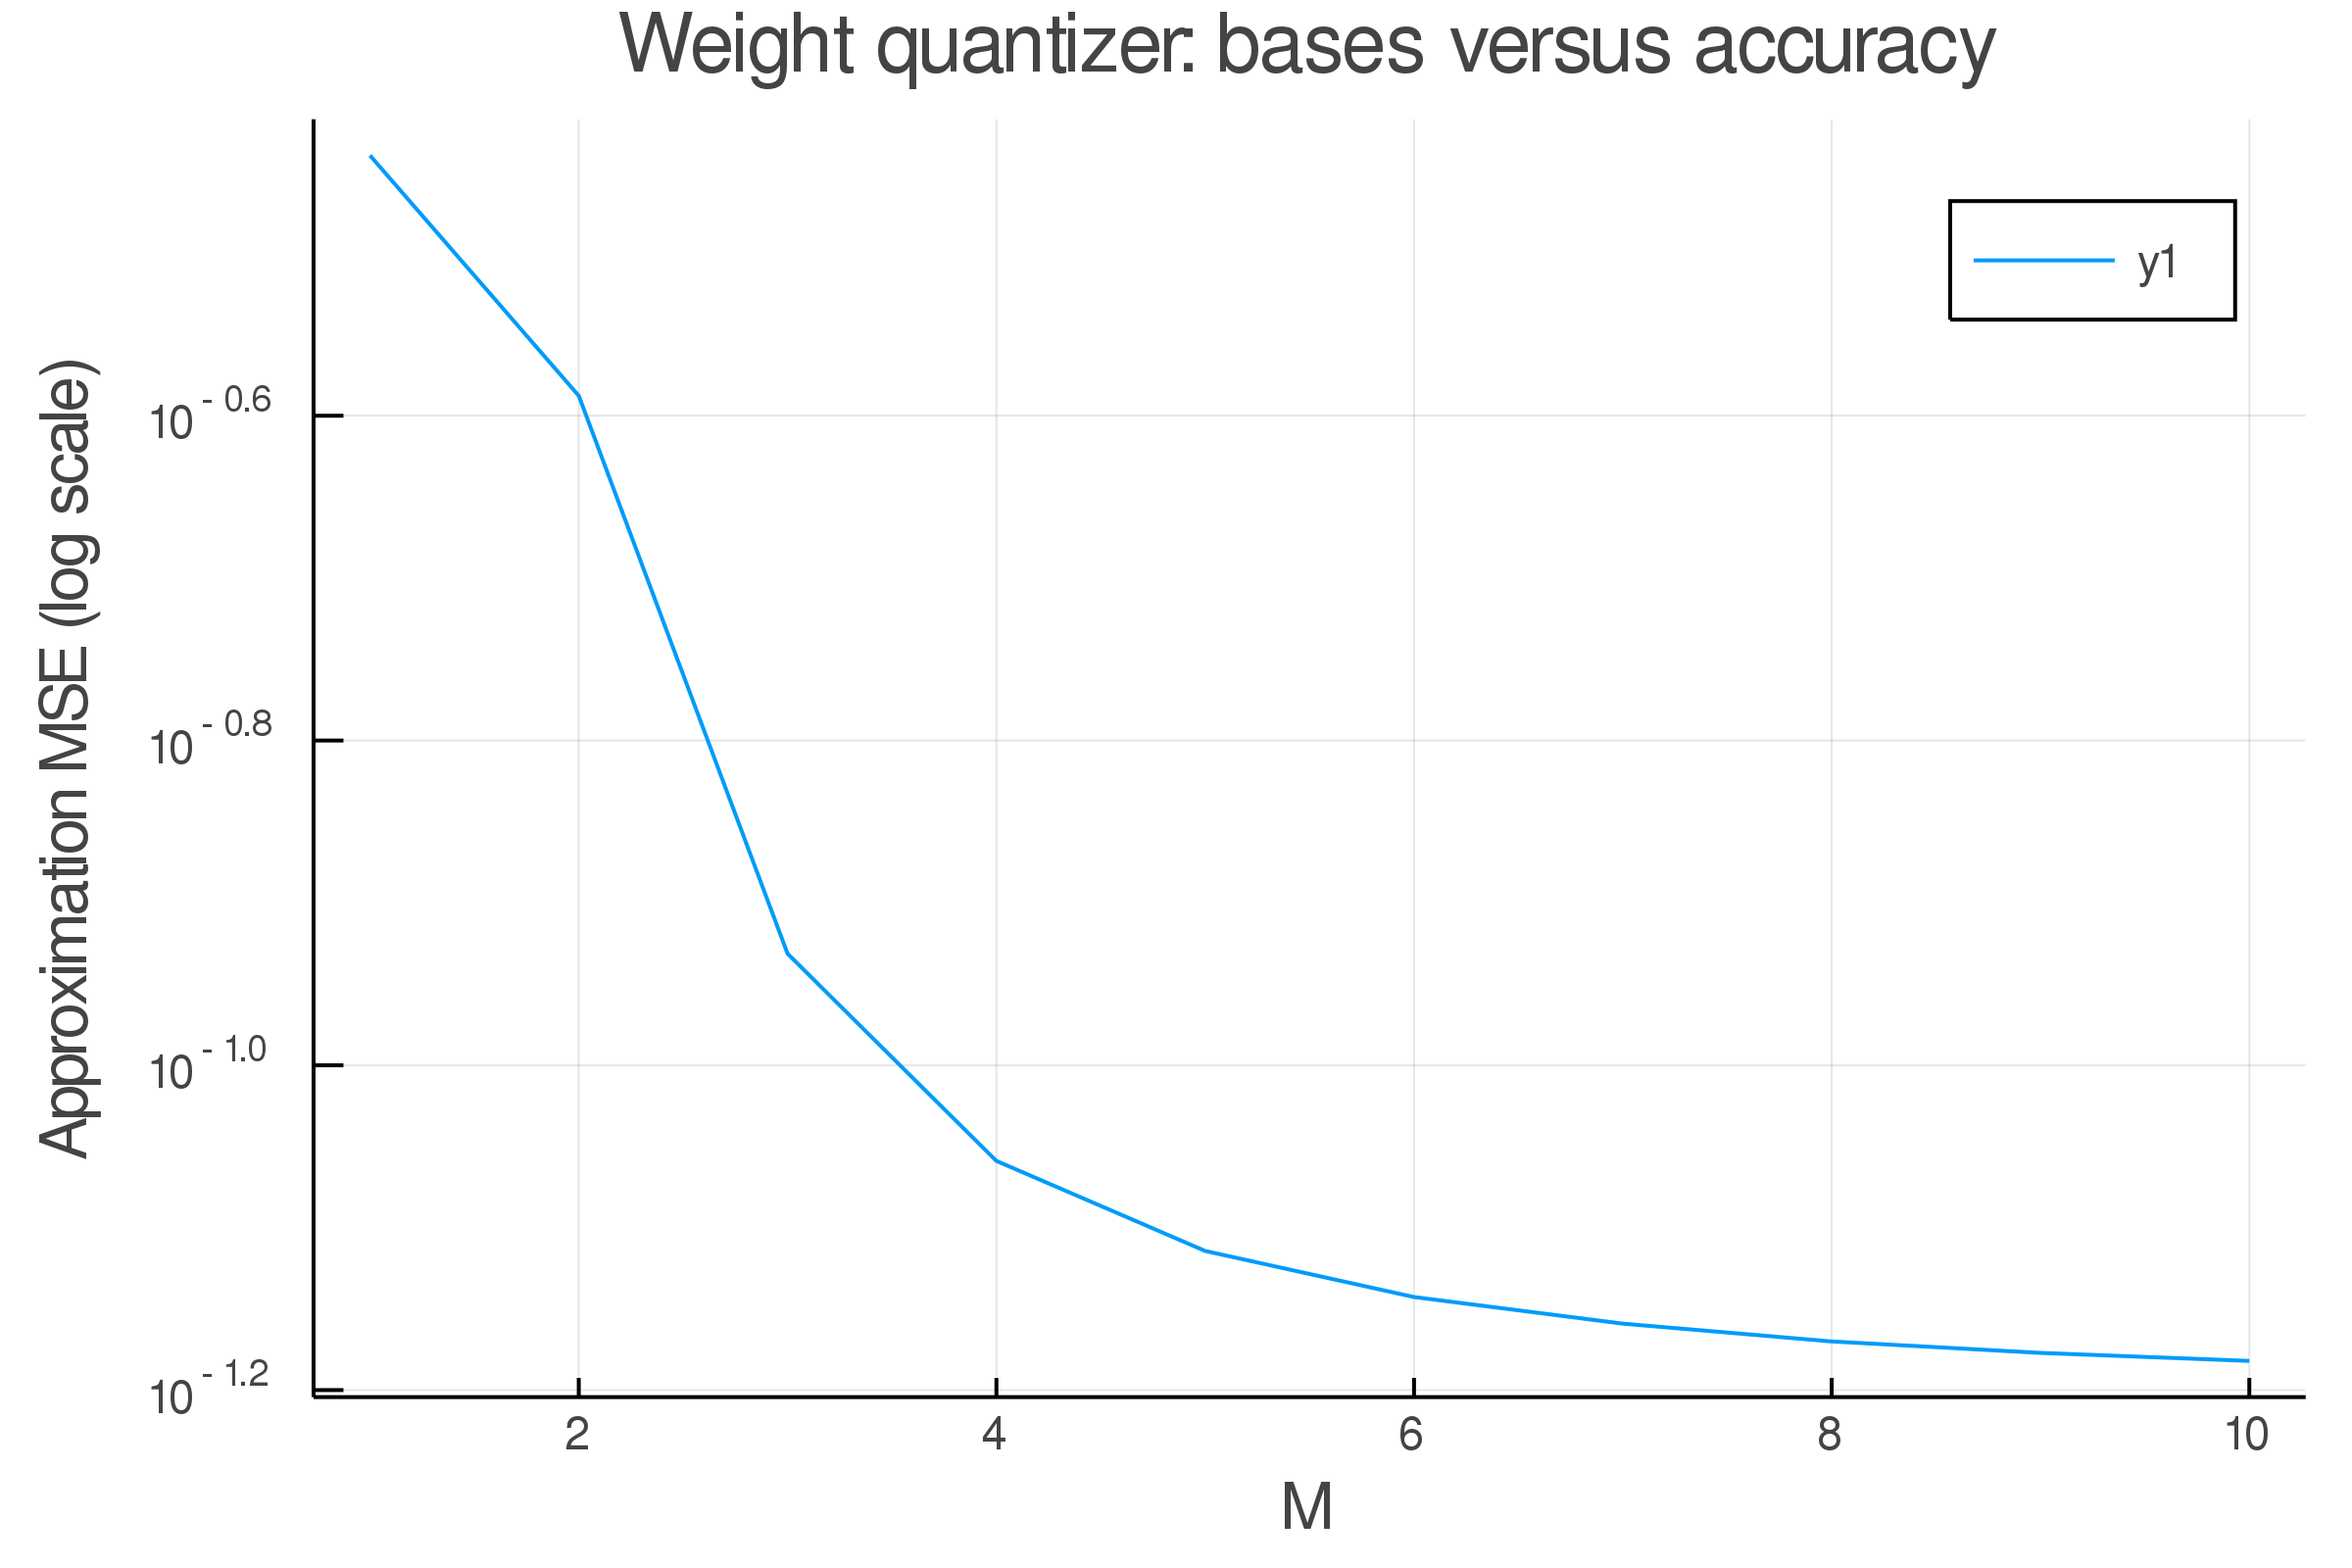
\includegraphics[width=5in]{./plots/weighttraining.png}
\end{center}

We see that the error lowers quickly as \(M\) increases, and then plateaus. It's possible that
the error could be decreased further by training the \(u_i\) parameters; that's a direction for future work.

The activation quantization must be trained through gradient descent. To test this, we train the quantization function on blocks of 10x10x10x10 normally distributed random activations, minimizing the MSE relative to the true activations using the Adam optimizer \citep{Adam}. In addition, we vary the number of bases available (\(N\)). (Note that each gradient descent step gives a \textbf{different} block of activations to approximate, with the same distribution parameters. This models varying activations during evaluation.)

\begin{center}
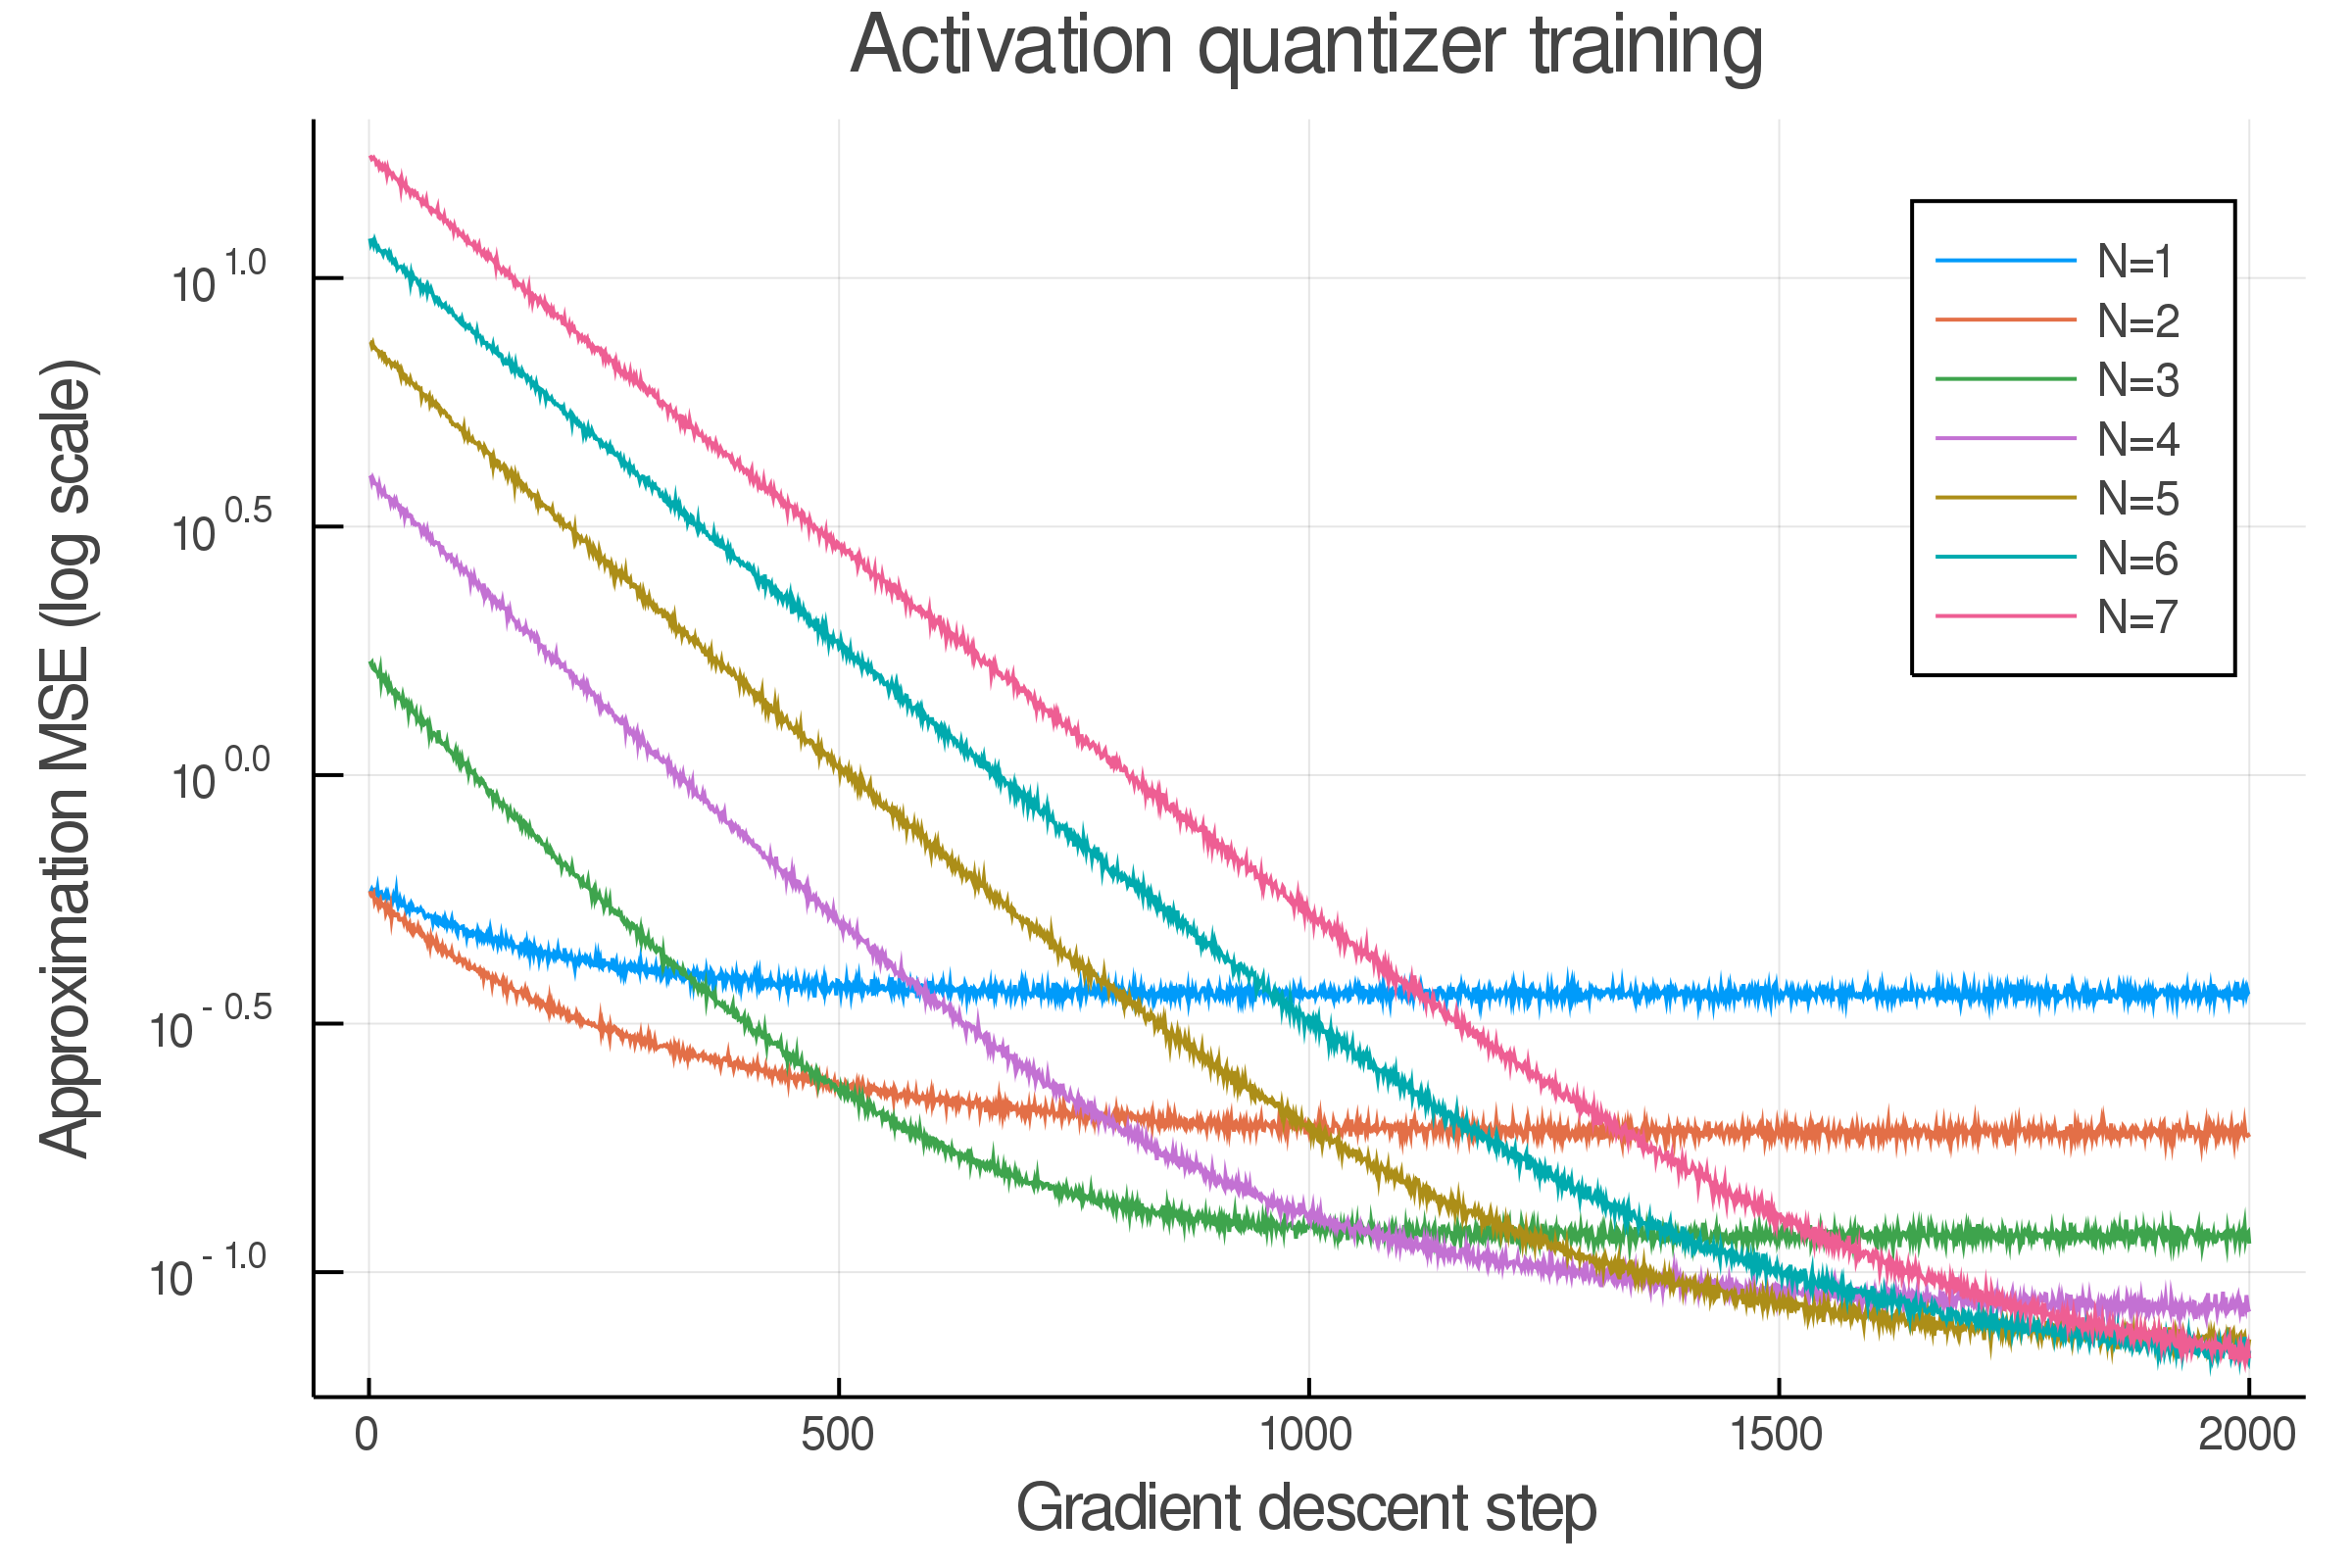
\includegraphics[width=5in]{./plots/acttraining.png}
\end{center}

We see that gradient descent is quite good at finding values for the activation quantization parameters. It's non-obvious that gradient should work in this case, when using the straight-through estimator, but it does.

(Do note that there isn't any MSE term in the actual loss during training; instead, the quantization is trained only to minimize the overall loss of the network. It's an open question whether adding other terms might improve performance.)

Finally, we implemented a floating point \texttt{ABCCrossCor} layer, which encapsulates quantizing weights and activations and then convolving (in floating point). Note that the operation called convolution in most neural network frameworks is actually cross correlation, since it doesn't flip the kernel along the X and Y axis. Flux bucks this trend by naming things correctly, and we follow suit.

We built a simple network using this layer and trained it on the FashionMNIST \citep{FashionMNIST} dataset, which is a dataset somewhere between MNIST and CIFAR in difficulty. The network is described as follows:

\begin{minted}[frame=lines,linenos=true,mathescape,breaklines=true,escapeinside=||]{julia}
N = 3
M = 3

model = Chain(
    CrossCor((3, 3), 1=>16, pad=(1,1)),
    BatchNorm(16), Relu(), ABCCrossCor((3, 3), 16=>32, N, M, pad=(1,1)),
    BatchNorm(32), Relu(), ABCCrossCor((3, 3), 32=>32, N, M, pad=(1,1)),
    MaxPool((2,2)),
    BatchNorm(32), Relu(), ABCCrossCor((3, 3), 32=>32, N, M, pad=(1,1)),
    BatchNorm(32), Relu(), ABCCrossCor((3, 3), 32=>64, N, M, pad=(1,1)),
    BatchNorm(64), Relu(), ABCCrossCor((3, 3), 64=>64, N, M, pad=(1,1)),
    MaxPool((2,2)),
    BatchNorm(64), Relu(), ABCCrossCor((3, 3), 64=>64, N, M, pad=(1,1)),
    BatchNorm(64), Relu(), ABCCrossCor((3, 3), 64=>64, N, M, pad=(1,1)),
    BatchNorm(64), Relu(), ABCCrossCor((3, 3), 64=>64, N, M, pad=(1,1)),
    MaxPool((2,2)),
    x -> reshape(x, :, size(x, 4)),
    Relu(),
    Dense(64 * 3 * 3, 10),
    softmax,
)
\end{minted}

Note that the first convolution is \textbf{not} quantized, which is standard in quantization studies. Additionally, we perform the BatchNorm + ReLU + quantize operation after max pooling, rather than before, on the recommendation of the original paper.

At full precision, this network achieves 93.1\% top-1 accuracy on the FashionMNIST dataset (when trained with the Adam optimizer using Flux default settings, input values in the range \((0, 1)\), and no data augmentation). When quantized and fine-tuned, the network achieves 91.0\% top-when accuracy, with M=N=3 bases for weights and activations.

\subsection{Packed Binary Operations}
\label{sec:org83ca12c}

The bulk of the work was spent implementing binary packing and convolution kernels using CUDAnative. CUDAnative imitates the CUDA C++ API. When implementing a CUDA program, the challenge is generally to achieve full utilization of all of the compute resources and memory bandwidth available on the device. There are many choices to be made, including how to map an input space to CUDA threads and CUDA blocks, how to coordinate between threads, and how to take advantage of shared memory.

First we implemented a quantization and packing kernel. This kernel is responsible for walking a \texttt{Float32} input tensor, applying a quantization operation to each input, and packing the resulting bits into a \texttt{UInt32} output tensor. We chose to pack into 32 bits instead of 64 in order to avoid \textbf{memory bank conflicts}, which will be discussed shortly. The quantization operation is user-supplied and fused into the kernel, which is easy to do because of how Julia and CUDAnative work.

This kernel also transposes the input.
All Flux operations for image processing keep their inputs in WHCB order: that is, x, y, channel, batch, with x walked first because Julia stores arrays in Fortran order. However, to ensure that results fit well into machine words we reordered this to PWHB in the kernel (packed channel, x, y, batch). In the case of multiple bases, the kernel splats the input out to a 5-dimensional array, PWHNB (packed channel, x, y, basis, batch).
(Keeping track of all these dimensions can be confusing. To avoid mistakes, we named all functions and variables based on their dimensions; for instance, the helper function that dispatches our quantization kernel is called \texttt{quant\_pack\_WHCB\_PWHNB\_32}.)

Bit-packing would seem to require communication between threads; that's slow. However, we were able to leverage the CUDA \texttt{vote\_ballot} intrinsic to make it extremely fast. CUDA thread blocks execute in "warps" of 32 threads; threads are grouped into warps by adjacent thread index.
The \texttt{vote\_ballot} intrinsic takes a boolean and returns an integer with bits set for every element in a warp. If the thread passed in \texttt{true}, the bit is 1; if the thread passed in \texttt{false}, the bit is 0. By carefully arranging the threads within our kernel, we ensure that warps line up with the regions of the input tensor that map to packed \texttt{UInt32s} in the output tensor. Then we used \texttt{vote\_ballot} to perform the required bit-packing in a single operation.

The performance of our quantization kernel is entirely bounded by global memory bandwidth. Within the kernel, there's very little communication or computation; just invocation of the quantization operation and a single \texttt{vote\_ballot} per output. The naive implementation turned out quite fast, so we didn't spend much time optimizing it.

We also implemented an unpacking kernel to check correctness of the packing kernel. We didn't optimize the unpacking kernel, though, since it isn't needed during model training or evaluation.

Finally, we implemented a binary "convolution" kernel. This kernel performs convolution (actually cross-correlation) between multiple bases of weights and activations, multiplies the results by the corresponding coefficients, and writes its output to a \texttt{Float32} tensor. To start, we implemented this as simply as possible. To verify correctness, we compared the results against CUDNN. CUDNN is an library of CUDA-accelerated neural network kernels from NVIDIA; it serves as Flux's built-in implementation for convolution. We also implemented a naive floating-point convolution kernel, arranged in the same structure as the binary kernel, to serve as a comparison.

This kernel was more interesting to optimize, since there was room for re-using intermediate memory accesses. CUDA provides a programmer-controlled shared memory space to each thread block, which behaves similarly to L1 cache. Our kernel was arranged so that all the threads in a thread block would re-use the same region of the input tensor. We therefore extended our kernel by having all the threads in each block start by collaboratively reading the relevant input region to the shared cache.

After that, we modified the iteration pattern of different threads to avoid bank conflicts. The shared memory cache has 32 access ports, arranged such that all the threads in a warp access adjacent 32-bit values, all the threads can read from separate ports. However, if some threads access the same value, those accesses must be serialized. We arranged our threads using what we termed a "barber pole pattern", where each thread started its iteration on a separate input region, and would remain mostly non-overlapping throughout.

\subsection{Benchmarks}
\label{sec:orgf142f29}
We benchmarked our kernels across a range of image sizes. Here's a comparison of our naive (floating-point) convolution kernel, and the corresponding quantized convolution kernel:

\begin{center}
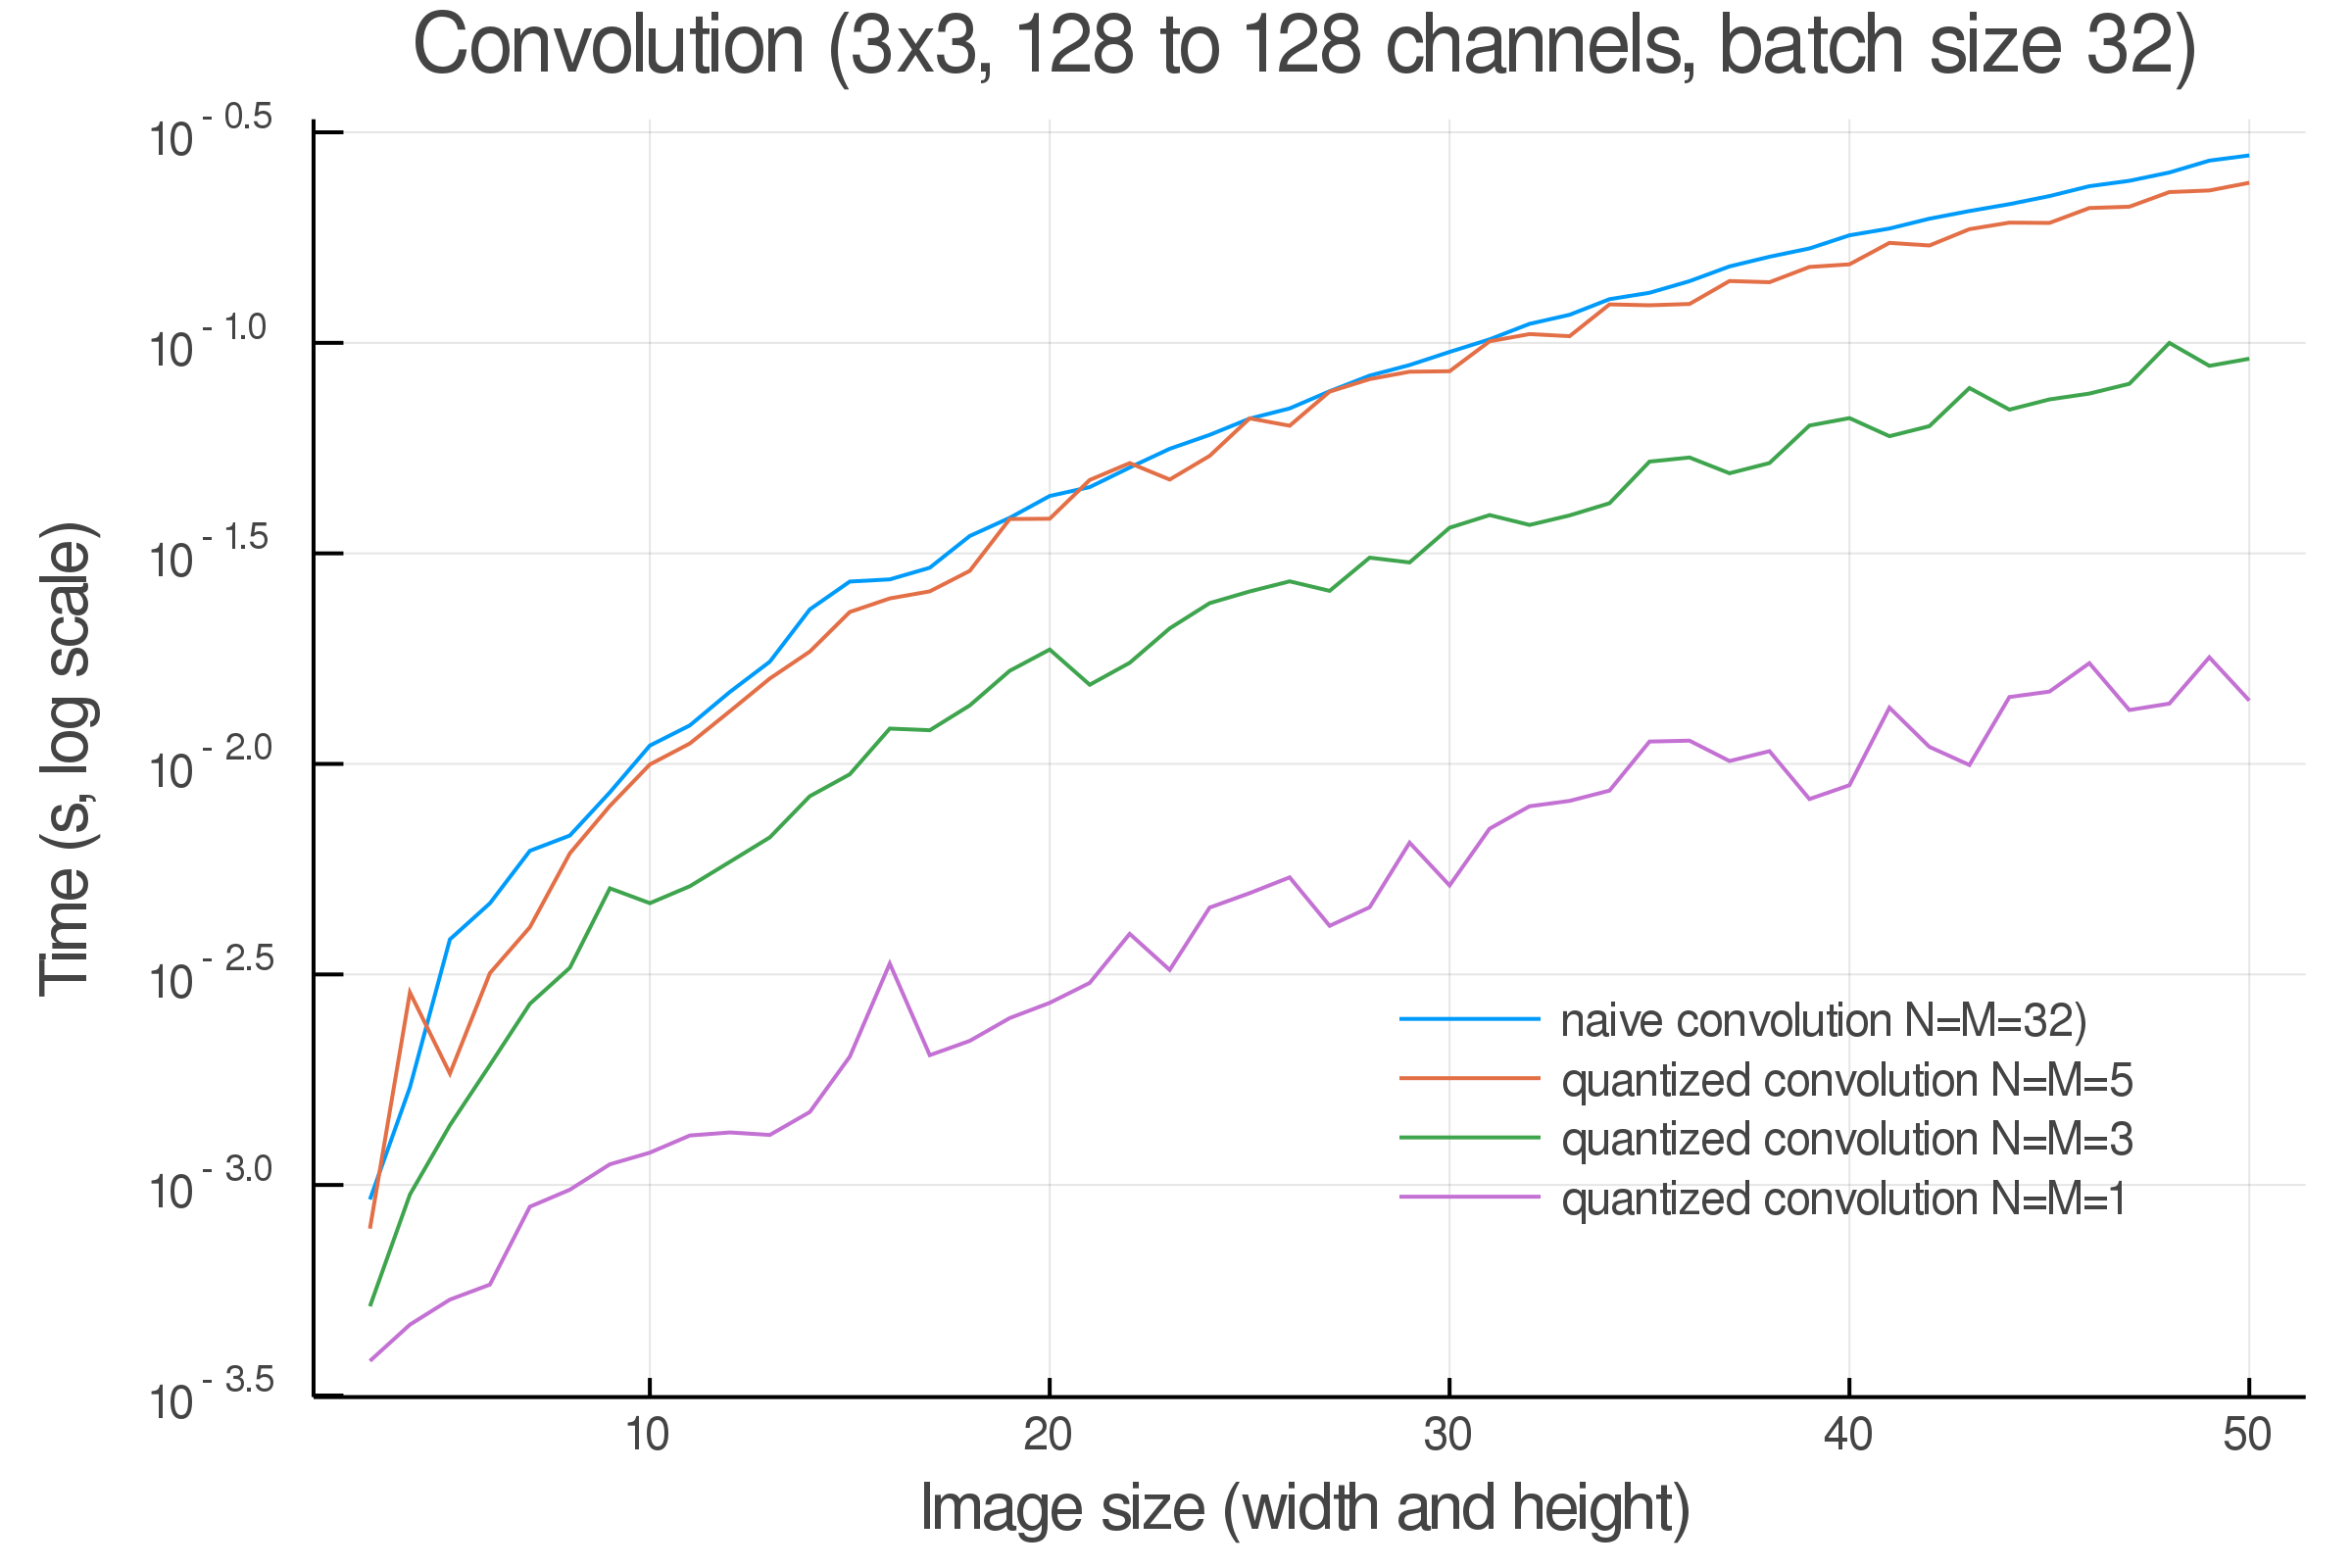
\includegraphics[width=5in]{./plots/varysizenocudnn.png}
\end{center}

This seems promising: lower precision quantization gives significant speedups. (Note the logarithmic time scale!) Unfortunately, it isn't the whole story. This is what happens when we add 32-bit CUDNN to the mix:

\begin{center}
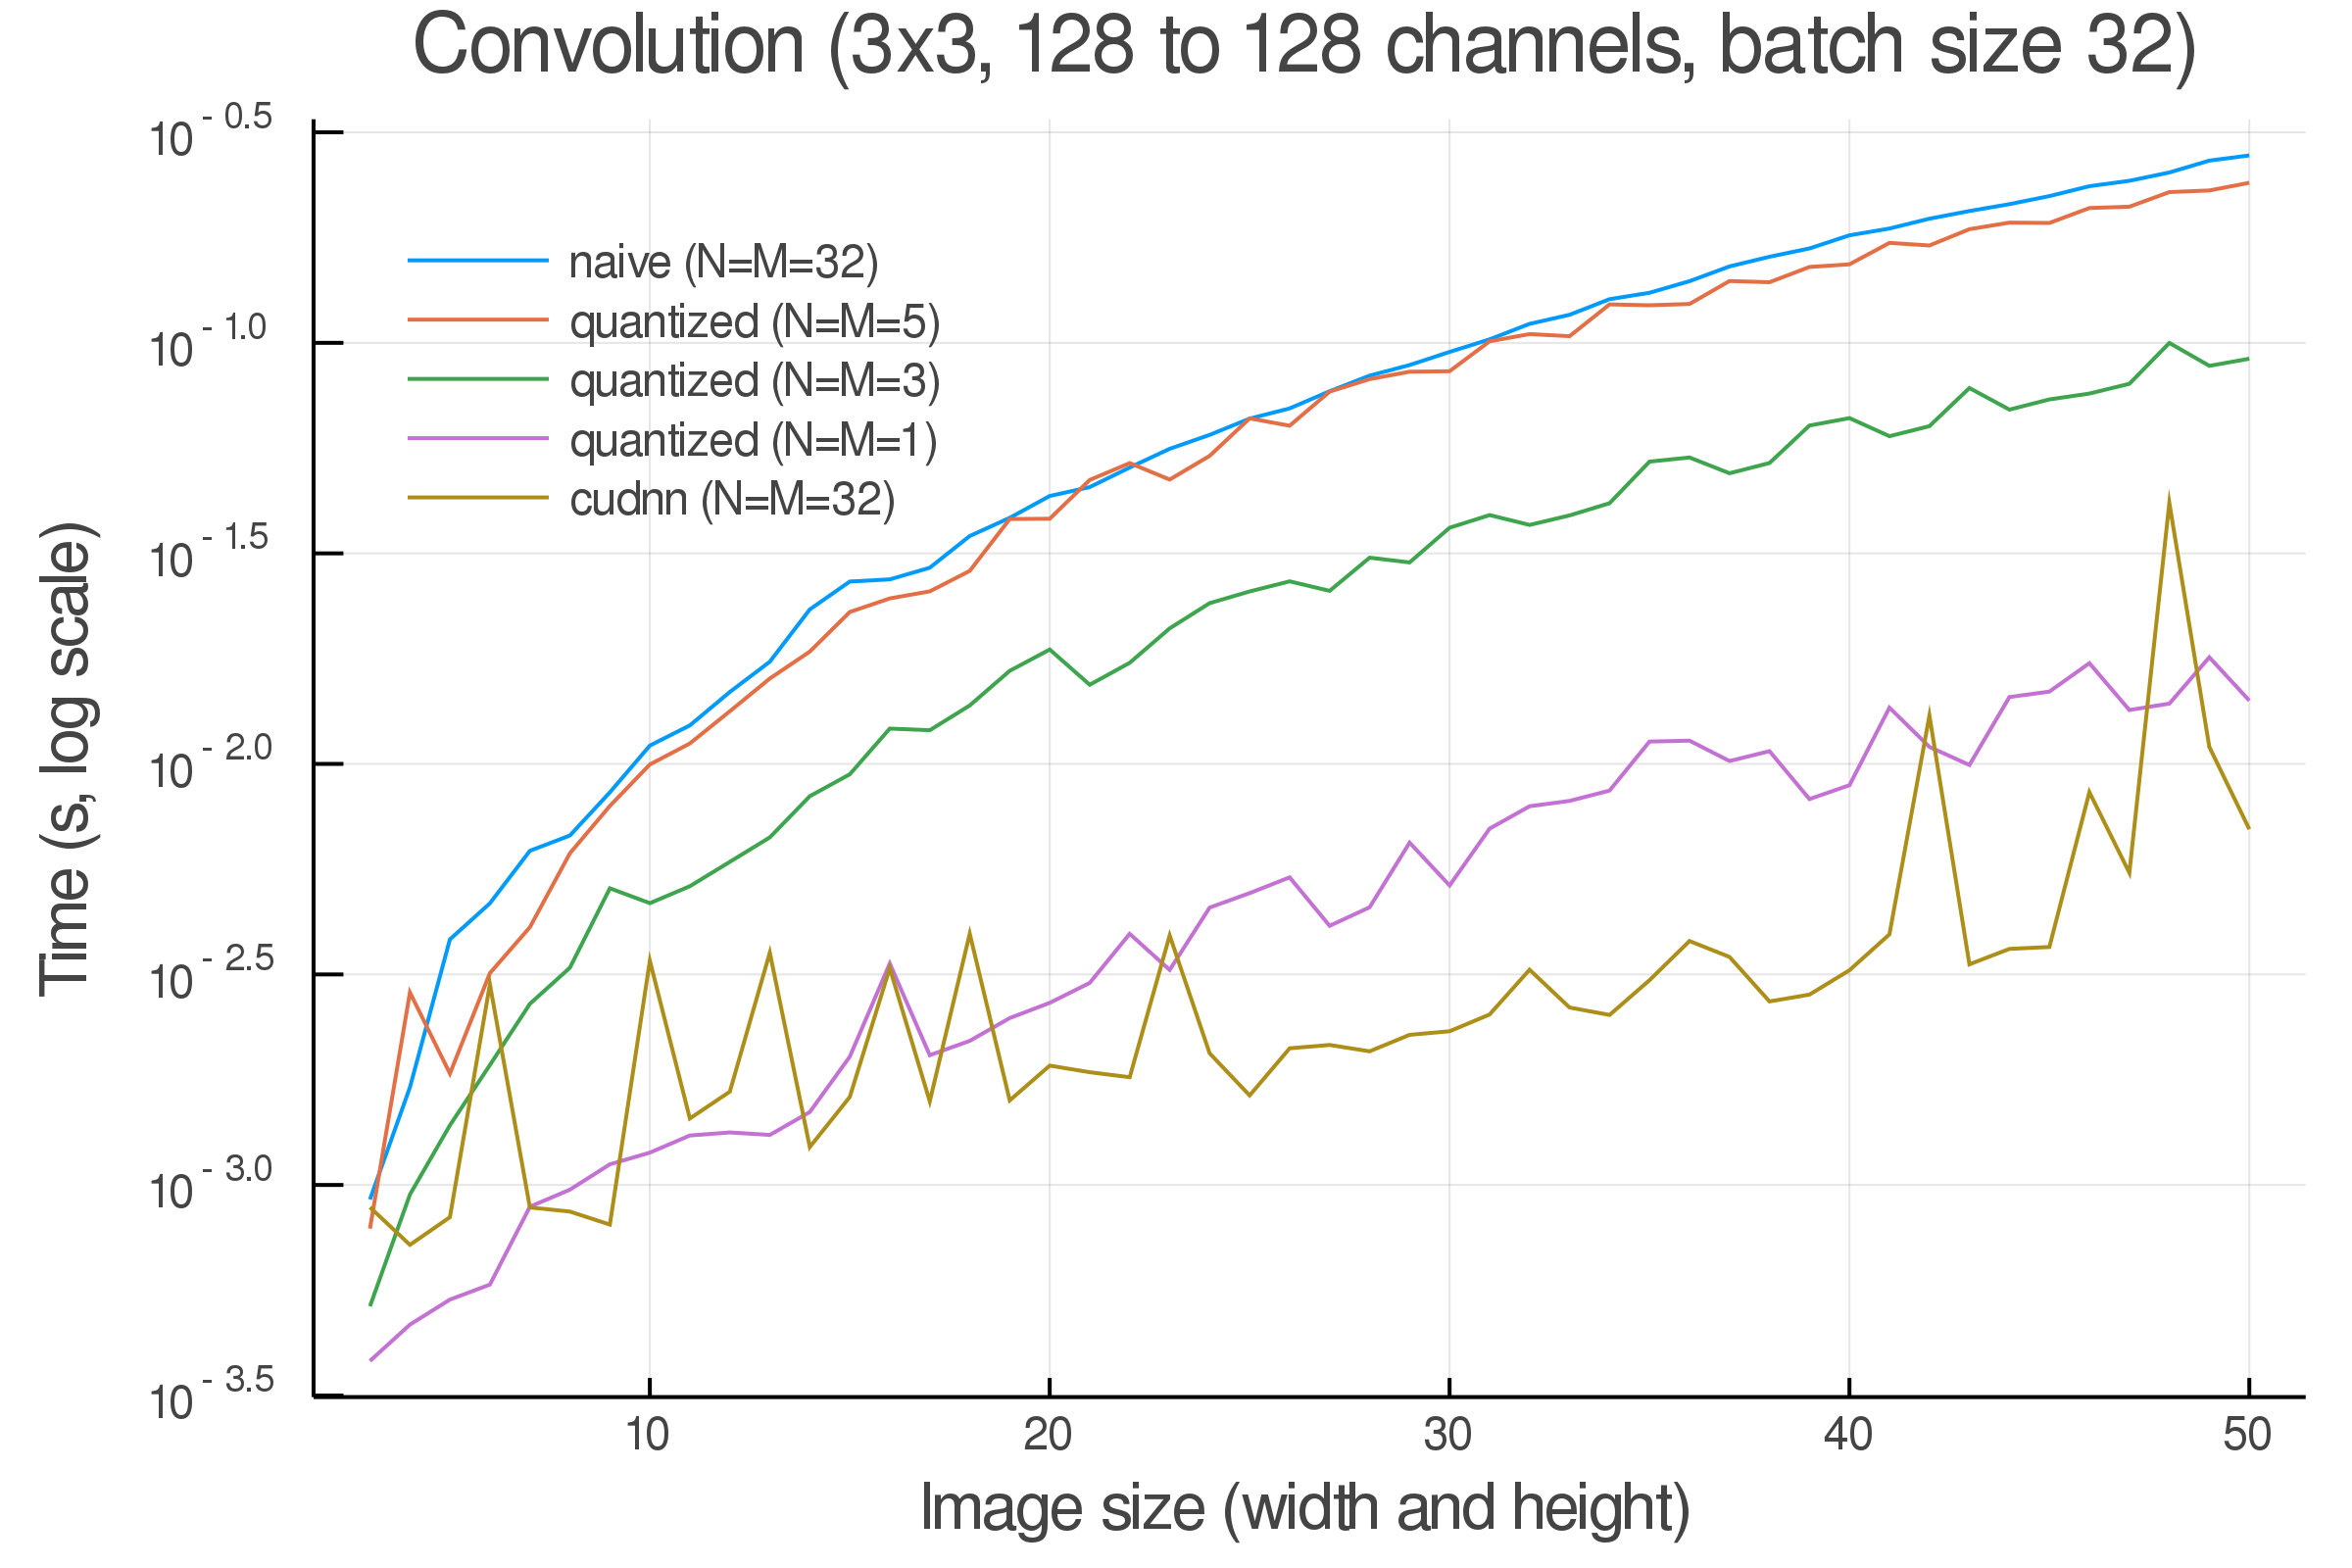
\includegraphics[width=5in]{./plots/varysizecudnn.png}
\end{center}

CUDNN beats even the binary version of our kernel! Why is that? Well, partially, CUDNN is just an extremely well-optimized library; but more importantly, we were \textbf{unable to use CUDA shared memory}. We ran into issues with our technical stack that prevented shared memory from providing any performance benefit, and were unable to fix these issues in time, despite days of debugging. In the end, we were forced to rip out the optimizations managing shared memory and iteration performance.

Still, we've shown that this algorithm can provide significant speedups over full precision. We hypothesize that we can wring major additional speedups out of the code once the issues preventing the use of shared memory are fixed; but for now, leave that to future work.

\section{Julia, CUDAnative.jl and Flux.jl: Benefits and Drawbacks}
\label{sec:orge49cc42}
In this section we reflect on how using Julia, CUDAnative, and Flux.

Some aspects of development were smooth and easy. Flux and CuArrays in particular provide an extremely elegant interface. For example, the floating-point implementation of equation (1) can be essentially copied from the equation listing, modulo some rearranging of axes:
\begin{minted}[frame=lines,linenos=true,mathescape,breaklines=true,escapeinside=||]{julia}
function weight_masks(W, us)
    dims = size(W)
    W̅ = W .- mean(W)
    std_W = std(W)
    W̃s = cat((sign.(W̅ .+ (u * std_W)) for u in us)...,
            dims=length(size(W)) + 1)
    W̃s
end
function binarize_weights(W, us)
    W̃s = weight_masks(W, us) # compute the masks of the weight tensor, given the u_i constants
    dims = size(W)
    Wv, W̃vs = reshape(W, :), reshape(W̃s, :, length(us)) # flatten weights and masks
    αs = W̃vs \ Wv # least squares
    W̃v = W̃vs * αs # compute result
    W̃ = reshape(W̃v, dims...) # reshape output
    # return (floating-point) approximated weights,
    # and the discovered optimal coefficients
    W̃, αs
end
Zygote.@adjoint function binarize_weights(W, us)
    W̃ = binarize_weights(W, us)
    # note: $\nabla$_W̃ should be read "gradient with respect to W̃"
    function adjoint((|$\nabla$|_W̃, |$\nabla$|_αs))
        # the straight-through estimator.
        # (us are not trainable.)
        (|$\nabla$|_W, |$\nabla$|_us) = (|$\nabla$|_W̃, nothing)
        (|$\nabla$|_W, |$\nabla$|_us)
    end
    W̃, adjoint
end
\end{minted}

Implementing the floating-point version was easy and resulted in very neat code, probably the most "mathematical" machine learning code the author has ever written. (Mathematical to a fault, in fact. One funny bug we found was that our convolution code only gave the same results as Flux when we flipped the kernel. This turned out to be because the Flux \texttt{Conv} layer performs \textbf{actual} convolution; we were looking for the operator wrongly referred to as convolution in most of the machine learning literature, which Flux correctly terms \texttt{CrossCor}).

CUDAnative was unfortunately significantly harder to work with. The primary issue was that some error in the tech stack caused a segfault when our code was run under \texttt{nvprof} and \texttt{nsys} (NVIDIA's tools for profiling CUDA code). It's not clear whether the issue is in the hardware we used, the OS, the driver, \texttt{nvprof}, or Julia itself. Despite several days of debugging, we were unable to resolve it. This meant that we were unable to acquire anything more than basic timing information for our kernels. This made optimizing the kernels extremely difficult, since we weren't sure where the bottlenecks were.

In addition, CUDAnative only supports a subset of Julia. For example, any code which calls string formatting implicitly relies on the Julia runtime, which CUDAnative will reject. This wouldn't seem like a huge problem, except that many error paths rely on string formatting to print errors. This means that a lot of seemingly innocuous code will cause CUDAnative to fail.
 This issue is compounded by the fact that CUDAnative's diagnostics can also be very difficult to understand. Often they aren't clear about which line of code caused an error, even when tools like \texttt{@device\_code\_warntype} is used.

These issues led to our being unable to use shared memory. We had to reimplement several tools from base Julia (such as \texttt{CartesianIndex}) and write some custom helper functions in order to copy chunks of our input arrays to shared memory. This code was \textbf{correct}; we were able to verify that it wrote and read the correct values. However, it didn't result in any speedup. Somewhere we were performing an operation that lacked mechanical sympathy. However, since we couldn't use a profiler, we didn't know which operation that was.

CUDAnative is extremely powerful, and allows many low-level operations to be implemented in ways that synchronize harmoniously with Flux and CuArrays. Unfortunately, some issues in the tech stack prevented us from using it to its full potential. Still, working on the project was very informative, and we look forward to leveraging this tech stack in the future once some of the kinks are ironed out.

\section{Future work}
\label{sec:org10fb8c9}
If we were to continue working on this project, we would first want to get shared memory working, perhaps by running the code under \texttt{nvprof} on several CUDA-enabled machines until we can find one that works.
After that, we'd like to optimize the kernels further, and then integrate our binary and floating point implementations, and see what optimizations that enables.
One optimization we're particularly curious about would be fusing the convolution, batchnorm, relu, and quantization kernels. This would mean that only packed bits would need to be written to global memory, with all floating-point numbers used in the kernel kept in shared memory, minimizing the necessary global memory bandwidth.

One other interesting direction of development would be the development of a tool like CUB (\url{https://nvlabs.github.io/cub/}) for Julia/CUDAnative. CUB provides a number of thread-cooperative algorithms that can be used directly within CUDA kernels. Having access to a tool like that would make CUDAnative significantly easier to use, and allow faster development of high-performance kernels.

\newpage
\bibliography{everything.bib}
\bibliographystyle{iclr2020_conference}
\end{document}
